
%%=============================================================================
%% H6 - ZPools & VDEV's
%%=============================================================================

\chapter{Zpools \& VDEV's}
\label{ch:h6}

In dit hoofdstuk worden zpools en diens bouwstenen, VDEV's, wat meer toegelicht. Er wordt ook een demonstratie gegeven over hoe men zpools en VDEV's aanmaakt en wijzigt.

\section{VDEV's: Virtual Devices}

\subsection{Concept}

VDEV's (of voluit Virtual Devices) zijn de bouwstenen van storage pools; het zijn een soort van device drivers die elk een bepaalde functionaliteit aanbieden. Er bestaan verschillende soorten VDEV's: zo zijn er bijvoorbeeld \gls{striping} VDEV's en mirror VDEV's. Ook worden de verschillende RAID-Z-vormen geïmplementeerd met behulp van één of meerdere VDEV's \autocite{ZFSBonwick}.

Conceptueel worden virtual devices voorgesteld in een boomstructuur, waarvan de bladeren de fysieke VDEV's voorstellen; deze VDEV's komen overeen met fysieke apparaten zoals harde schijven. De andere knopen in de boom worden logische VDEV's genoemd omdat ze een groepering vormen van fysieke VDEV's. Zoals in elke boom bestaat er ook in deze structuur van virtual devices een wortel of \textit{root}. De kinderen van deze root VDEV worden de top-level VDEV's genoemd \autocite{Microsystems2006}.

\begin{figure}
  \centering
  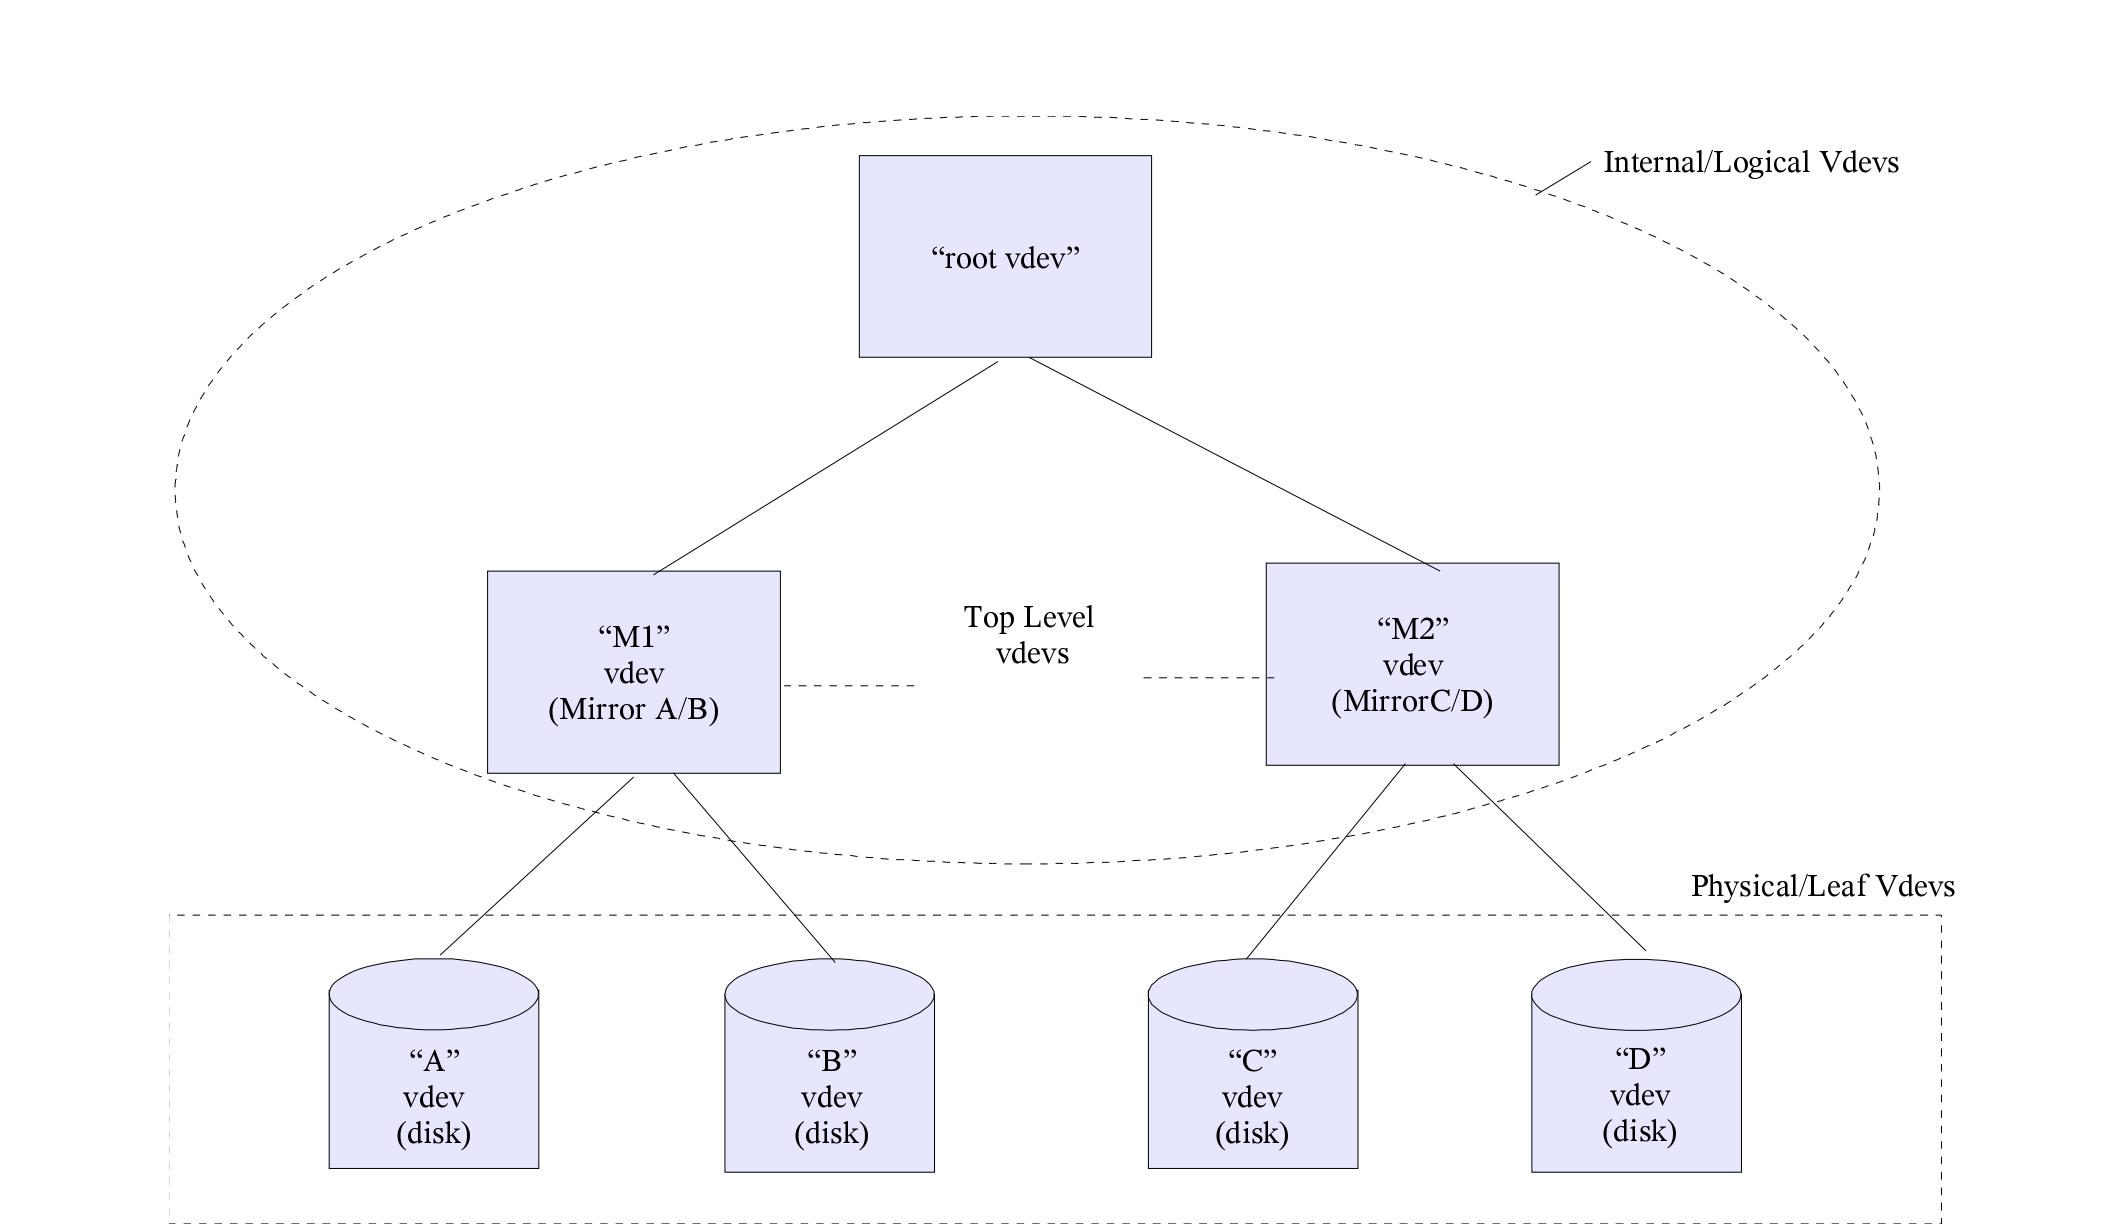
\includegraphics[width=0.9\textwidth]{h6_vdevs_tree}
  \caption{Conceptuele voorstelling van VDEV's in een boomstructuur: M1 en M2 zijn mirrors VDEV's; apparaten A t.e.m. D zijn kinderen van deze VDEV's \autocite{Microsystems2006}.}
  \label{fig:vdevs_boom}
\end{figure}

\subsection{Speciale VDEV's}

Naast VDEV's voor redundantie en \gls{striping} bestaan er ook nog andere virtual devices die een specifieke rol vervullen. Deze VDEV's worden ingezet met als hoofddoel de \gls{performantie} van ZFS naar omhoog te trekken \autocite{Lucas2015}.

\subsubsection{SLOG: Seperate Intent Log}

Onder normale omstandigheden bevindt de ZFS Intent Log (ZIL) zich in een pool en worden de bewerkingen die op dit moment bezig zijn naar deze log geschreven. Echter kan de systeembeheerder deze log naar een apart, snel apparaat (zoals een SSD) buiten een pool verplaatsen om zo de \gls{performantie} omhoog te trekken. ZFS kan logdata effciënter groeperen in batches in plaats van deze weg te schrijven in de volgorde dat de opslagbewerkingen gebeuren; daarna worden deze weggeschreven naar de pool. Dit verhoogt de gehele efficiëntie en snelheid van bewerkingen aanzienlijk. Vele databanksystemen wachten bijvoorbeeld totdat data gepersisteerd is naar de schijf alvorens verder te gaan met een volgende operatie. ZFS kan deze soort operaties loggen en achteraf uitvoeren; het bestandssysteem meldt terwijl aan de databank dat deze operatie gepersisteerd is \autocite{Lucas2015}.

\subsubsection{L2ARC: Level 2 Adaptive Replacement Cache}

Traditioneel gebruiken schijven en bestandssystemen buffers of caches om veelgebruikte data tijdelijk bij te houden; bestandssystemen gebruiken het RAM geheugen om blokken data tijdelijk bij te houden \autocite{OSThreePiecesRemzi2015}. ZFS is hierop geen uitzondering en cachet ook data in het werkgeheugen. Naast dze vorm van caching beschikt ZFS ook over de Adaptive Replacement Cache (ARC). Dit geeft de mogelijkheid om een snel apparaat (zoals een SSD) te gebruiken als extra cache om veelgebruikte bestanden in op te slaan. Het grote verschil met deze manier van bufferen en het gebruik van caches in het RAM-geheugen, is dat in de L2ARC (Level 2 ARC) enkel bestanden worden bijgehouden die frequent gebruikt worden, maar dan weer niet frequent genoeg om in het werkgeheugen te worden bijgehouden \autocite{Lucas2015}. 

\section{Storage pools of zpools}

Zoals reeds gezegd in Hoofdstuk \ref{ch:h3} vormen storage pools (of zpools in ZFS-termen) de eerste vorm van abstractie binnen de gehele ZFS-stack: zpools bieden namelijk een interface aan tot de onderliggende fysieke schijven. Het zijn echter VDEV's die ervoor zorgen dat data kan weggeschreven worden van en naar de schijven. Ter verduidelijking kan er een analogie worden gemaakt met een traditionele RAID-controller en de schijven in een RAID-array: zpools vervullen de rol van RAID-controller, terwijl VDEV's de schijven van de 'array' voorstellen. De zpool ('RAID-controller') verdeelt of stripet data over één of meerdere VDEV's ('schijven') \autocite{Lucas2015}.

\subsection{Aanmaken en beheren van zpools}

Het testsysteem waarover we beschikken bevat drie interne harde schijven, elk direct aangesloten op het moederbord met een SATA-kabel. Dit aantal is voldoende om een RAID-Z1 opstelling mee te maken. Vooraleer er echter VDEV's kunnen worden toegevoegd of gewijzigd, moet er eerst een ZFS storage pool worden aangemaakt; er kunnen meerdere storage pools worden aangemaakt, maar in ons geval is één storage pool meer dan voldoende.

\subsubsection{Bekijken van aanwezige pools}

Voor het beheer van pools wordt er gebruik gemaakt van het commando \texttt{zpool}. Om bijvoorbeeld de huidige zpools te bekijken, geeft men het volgende commando in:

\begin{lstlisting}[language=bash,style=command_style]
$ zpool list
no pools available
\end{lstlisting}

\subsubsection{Aanmaken van een nieuwe pool}

Op dit moment zijn er nog geen pools aangemaakt, dus de uitvoer van bovenstaand commando is normaal. Om een zpool aan te maken met de drie schijven waarover we beschikken, gebruik je het volgende commando:

\begin{lstlisting}[language=bash,style=command_style]
$ zpool create storage /dev/sda /dev/sdb /dev/sdc
\end{lstlisting}

\clearpage

Deze instructie maakt een zpool aan met de naam 'storage'. Vervolgens kan je een lijst opvragen van alle pools die op het systeem aanwezig zijn:

\begin{lstlisting}[language=bash,style=command_style]
$ zpool list
NAME      SIZE  ALLOC   FREE  EXPANDSZ   FRAG    CAP  DEDUP  HEALTH 
storage  2.27T   154K  2.27T         -     0%     0%  1.00x  ONLINE 

(deel van de uitvoer is weggelaten)

\end{lstlisting}

De uitvoer van dit commando geeft reeds enkele eigenschappen van de pool weer, zoals de naam, de totale grootte van de pool, de gebruikte ruimte van de pool, de vrije ruimte en de hoeveelheid fragmentatie. Een andere eigenschap die interessant kan zijn, is DEDUP of deduplicatie: indien er verschillende kopieën zijn van een stuk data, dan houdt ZFS deze maar één keer bij. 

\subsubsection{Gezondheid van pools}

Om de gezondheid en structuur van een pool na te kijken, gebruik je het commando \texttt{zpool status}:

\begin{lstlisting}[language=bash,style=command_style]
$ zpool status
  pool: storage
 state: ONLINE
  scan: none requested
config:

	NAME        STATE     READ WRITE CKSUM
	storage     ONLINE       0     0     0
	  sda       ONLINE       0     0     0
	  sdb       ONLINE       0     0     0
	  sdc       ONLINE       0     0     0

errors: No known data errors
\end{lstlisting}

Dit commando geeft een overzicht van de interne structuur en gezondheid van elke pool op het systeem, samen met de aanwezige VDEV's. Het merendeel van de uitvoer spreekt voor zich: 'pool' geeft de naam van de pool weer en 'state' geeft de algemene toestand van een pool weer. De eigenschap 'scan' geeft aan of er een zogenaamde scrub wordt uitgevoerd of uitgevoerd is geweest. Een scrub is een scan die kan worden uitgevoerd door ZFS om de consistentie en integriteit van de pool na te gaan; indien mogelijk worden fouten automatisch gerepareerd. Een scrub is dus in principe de equivalent voor een \texttt{\gls{fsck}} binnen ZFS. De vijf kolommen onder de eigenschap 'config' geven informatie over de VDEV's van de pool weer; de drie kolommen aan de rechterzijde geven het aantal fouten aan dat door een bepaald VDEV werd gedetecteerd.

\subsubsection{Eigenschappen van pools}

Zoals reeds gezegd in Hoofdstuk \ref{ch:h3} is ZFS grotendeels een objectgeoriënteerd bestandssysteem. Elk object binnen ZFS heeft bepaalde eigenschappen (properties); deze kunnen dan ook worden opgehaald en gewijzigd. Het is dan ook niet verwonderlijk dat zpools tevens objecten zijn, met elk bepaalde eigenschappen.

Om bijvoorbeeld alle eigenschappen van een pool op te halen, gebruikt men het commando \texttt{zpool get all <naam van de pool>}:

\begin{lstlisting}[language=bash,style=command_style]
$ zpool get all storage
NAME     PROPERTY         VALUE                   SOURCE
storage  size             2.27T                   -
storage  capacity         0%                      -
storage  altroot          -                       default
storage  health           ONLINE                  -
storage  guid             2498162094782357460     default
storage  version          -                       default
storage  bootfs           -                       default
storage  delegation       on                      default
storage  autoreplace      off                     default
storage  cachefile        -                       default
storage  failmode         wait                    default
storage  listsnapshots    off                     default

(deel van de uitvoer is weggelaten)
\end{lstlisting}

Indien men een eigenschap van een pool wilt wijzigen, gebruikt men het commando \texttt{zpool set <eigenschap>=<waarde> <naam van de pool>}: 

\begin{lstlisting}[language=bash,style=command_style]
$ zpool set comment="Testpool" storage
$ zpool get comment storage
NAME     PROPERTY  VALUE     SOURCE
storage  comment   Testpool  local
\end{lstlisting}

In bovenstaand voorbeeld werd de property 'comment' aangepast; vervolgens werd de nieuwe waarde opgehaald.

\subsubsection{Verwijderen van een pool}

Om een zpool en diens VDEV's te verwijderen, gebruik je het commando \texttt{zpool destroy <naam van de pool>}:

\begin{lstlisting}[language=bash,style=command_style]
$ zpool destroy storage
$ zpool list
no pools available
\end{lstlisting}

\clearpage

\subsection{Aanmaken en wijzigen van VDEV's}

In het begin van dit hoofdstuk werd er reeds kort gesproken over VDEV's en hun rol bij zpools: alle redundantie bij RAID-Z zit in feite in deze VDEV's. Het zijn de virtual devices (en dus niet de storage pools) die het maken van een RAID-opstelling binnen ZFS mogelijk maken \autocite{Lucas2015}.

De eigenschappen en principes van de verschillende soorten redundantie VDEV's komen grotendeels overeen met de overeenkomstige standaard RAID-niveaus; deze werden reeds uitvoerig besproken in Hoofdstuk \ref{ch:h2}.

Vooraleer er overgegaan wordt tot het aanmaken van VDEV's, moet er worden opgemerkt dat de structuur van zpools en van de meeste VDEV's na creatie vast ligt. Zpools kunnen uitgebreid worden met meer schijven en/of partities en VDEV's, maar aan een VDEV kan men in de meeste gevallen geen apparaten toevoegen \autocite{FBSDDP2017}. 

\subsubsection{Striping VDEV's}

Striping VDEV's komen overeen met RAID-niveau 0; bij zpools bestaande uit \gls{striping} VDEV's wordt data gelijkmatig verdeeld over de verschillende VDEV's.

In de voorgaande sectie over zpools werden er bij het aanmaken van een nieuwe zpool impliciet \gls{striping} VDEV's gebruikt:

\begin{lstlisting}[language=bash,style=command_style]
$ zpool create storage /dev/sda /dev/sdb /dev/sdc
$ zpool status
  pool: storage
  state: ONLINE
  scan: none requested
  config:

	NAME        STATE     READ WRITE CKSUM
	storage     ONLINE       0     0     0
	  sda       ONLINE       0     0     0
	  sdb       ONLINE       0     0     0
	  sdc       ONLINE       0     0     0

  errors: No known data errors
\end{lstlisting}

In dit geval wordt elke fysieke harde schijf in een aparte VDEV gestopt en wordt de data gelijkmatig verdeeld over de drie VDEV's (\texttt{sda}, \texttt{sdb} en \texttt{sdc}).

\subsubsection{Mirror VDEV's}

Bij mirror VDEV's zijn de kinderen van de VDEV's kopieën van elkaar: dit is hetzelfde principe dat bij RAID 1 wordt toegepast. 

Mirrors zijn overigens de enige VDEV's waaraan die men na creatie nog kan wijzigen, samen met stripes. Aan een mirror VDEV kunnen achteraf nog schijven worden toegevoegd; een \gls{striping} VDEV kan worden geüpgradet tot een mirror VDEV door een extra schijf of schijven aan de VDEV toe te voegen \autocite{FBSDDP2017}.

We beschikken bijvoorbeeld over de volgende storage pool met één \gls{striping} VDEV, bestaande uit één fysieke schijf:

\begin{lstlisting}[language=bash,style=command_style]
$ zpool create storage /dev/sda
$ zpool status
  pool: storage
  state: ONLINE
  scan: none requested
  config:

	NAME        STATE     READ WRITE CKSUM
	storage     ONLINE       0     0     0
	  sda       ONLINE       0     0     0

  errors: No known data errors
\end{lstlisting}

Deze \gls{striping} VDEV kan makkelijk worden geüpgradet naar een mirror VDEV m.b.v. het commando \texttt{zpool attach <naam pool> <naam VDEV> <schijf>}:

\begin{lstlisting}[language=bash,style=command_style]
$ zpool attach storage sda sdb
$ zpool status
  pool: storage
  state: ONLINE
  scan: resilvered 59.5K in 0h0m with 0 errors on Tue May  9 17:16:23 2017
  config:

	NAME        STATE     READ WRITE CKSUM
	storage     ONLINE       0     0     0
	  mirror-0  ONLINE       0     0     0
	    sda     ONLINE       0     0     0
	    sdb     ONLINE       0     0     0

  errors: No known data errors
\end{lstlisting}

Bij het weergeven van de structuur van de pool, kan men zien dat de stripe werd geüpgradet naar een mirror, met \texttt{sda} en \texttt{sdb} als kinderen. Ook werd er een scrub uitgevoerd na het toevoegen van de nieuwe schijf.

\subsubsection{RAID-Z1 VDEV's}

Aangezien het testsysteem over slechts drie fysieke schijven beschikt, kunnen we niet verder gaan dan RAID-niveau 5\footnote{In theorie zou er kunnen gebruikt gemaakt worden van binary files als storage-backend; ZFS kan namelijk bestanden gebruiken als provider. Maar aangezien deze bestanden op de externe harde schijf zouden moeten worden opgeslagen, zou dit de \gls{performantie} te sterk naar beneden halen (de schijf is aangesloten via USB 2.0).}. Het equivalent van RAID 5 bij ZFS is RAID-Z1.  

Om een RAID-Z1 VDEV te kunnen creeëren, dienen eerst de bestaande VDEV's worden verwijderd. Het makkelijkste is om de bestaande pool volledig te verwijderen en een nieuwe pool met een RAID-Z1 VDEV aan te maken:

\begin{lstlisting}[language=bash,style=command_style]
$ zpool destroy storage
$ zpool create storage raidz1 /dev/sda /dev/sdb /dev/sdc
$ zpool status
  pool: storage
  state: ONLINE
  scan: none requested
  config:

	NAME        STATE     READ WRITE CKSUM
	storage     ONLINE       0     0     0
	  raidz1-0  ONLINE       0     0     0
	    sda     ONLINE       0     0     0
	    sdb     ONLINE       0     0     0
	    sdc     ONLINE       0     0     0

  errors: No known data errors
\end{lstlisting}

Er zijn nog andere RAID-Z VDEV's mogelijk, zoals RAID-Z2 (equivalent van RAID 6) en RAID-Z3. Deze vereisen echter vier schijven of meer en zijn dus niet mogelijk in combinatie met het testsysteem.

\subsubsection{SLOG \& L2ARC VDEV's}

Typisch wordt er een klein en snel opslagapparaat - zoals een SSD - gebruikt voor de SLOG en L2ARC. Om te demonstreren hoe de indeling van een pool met één van deze VDEV's er zou uitzien, wordt er telkens een mirror VDEV aangemaakt samen met respectievelijk een SLOG VDEV en een L2ARC VDEV. Een SLOG VDEV kan worden gemirrored; een L2ARC VDEV niet \autocite{FBSDDP2017}.

Eerst en vooral moet de bestaande pool worden verwijderd; nadien kan een nieuwe pool met de nodige VDEV's worden aangemaakt:

\begin{lstlisting}[language=bash,style=command_style]
$ zpool destroy storage
$ zpool create storage mirror /dev/sda /dev/sdb log /dev/sdc
$ zpool status
  pool: storage
 state: ONLINE
  scan: none requested
config:

	NAME        STATE     READ WRITE CKSUM
	storage     ONLINE       0     0     0
	  mirror-0  ONLINE       0     0     0
	    sda     ONLINE       0     0     0
	    sdb     ONLINE       0     0     0
	logs
	  sdc       ONLINE       0     0     0

  errors: No known data errors
\end{lstlisting}

In bovenstaand voorbeeld ziet men mooi dat SLOG VDEVS zich buiten een pool bevinden. Ook is er in dit geval een duidelijk onderscheid tussen logische en fysieke VDEV's: \texttt{mirror-0} en \texttt{logs} zijn logische VDEV's, terwijl \texttt{sda}, \texttt{sdb} en \texttt{sdc} fysieke VDEV's zijn. Men ziet ook dat het mogelijk is om bij de creatie van een pool onmiddellijk alle VDEV-definities mee te geven.

Het aanmaken van een caching VDEV verloopt gelijkaardig:

\begin{lstlisting}[language=bash,style=command_style]
$ zpool destroy storage
$ zpool create storage mirror /dev/sda /dev/sdb cache /dev/sdc
$ zpool status
  pool: storage
 state: ONLINE
  scan: none requested
config:

	NAME        STATE     READ WRITE CKSUM
	storage     ONLINE       0     0     0
	  mirror-0  ONLINE       0     0     0
	    sda     ONLINE       0     0     0
	    sdb     ONLINE       0     0     0
	cache
	  sdc       ONLINE       0     0     0

  errors: No known data errors
\end{lstlisting}

Ook hier bevindt de L2ARC VDEV zich buiten de pool en kan opnieuw de indeling tussen fysieke en logische VDEV's duidelijk worden opgemerkt.
